% Options for packages loaded elsewhere
\PassOptionsToPackage{unicode}{hyperref}
\PassOptionsToPackage{hyphens}{url}
%
\documentclass[
  man,floatsintext]{apa7}
\usepackage{amsmath,amssymb}
\usepackage{iftex}
\ifPDFTeX
  \usepackage[T1]{fontenc}
  \usepackage[utf8]{inputenc}
  \usepackage{textcomp} % provide euro and other symbols
\else % if luatex or xetex
  \usepackage{unicode-math} % this also loads fontspec
  \defaultfontfeatures{Scale=MatchLowercase}
  \defaultfontfeatures[\rmfamily]{Ligatures=TeX,Scale=1}
\fi
\usepackage{lmodern}
\ifPDFTeX\else
  % xetex/luatex font selection
\fi
% Use upquote if available, for straight quotes in verbatim environments
\IfFileExists{upquote.sty}{\usepackage{upquote}}{}
\IfFileExists{microtype.sty}{% use microtype if available
  \usepackage[]{microtype}
  \UseMicrotypeSet[protrusion]{basicmath} % disable protrusion for tt fonts
}{}
\makeatletter
\@ifundefined{KOMAClassName}{% if non-KOMA class
  \IfFileExists{parskip.sty}{%
    \usepackage{parskip}
  }{% else
    \setlength{\parindent}{0pt}
    \setlength{\parskip}{6pt plus 2pt minus 1pt}}
}{% if KOMA class
  \KOMAoptions{parskip=half}}
\makeatother
\usepackage{xcolor}
\usepackage{graphicx}
\makeatletter
\def\maxwidth{\ifdim\Gin@nat@width>\linewidth\linewidth\else\Gin@nat@width\fi}
\def\maxheight{\ifdim\Gin@nat@height>\textheight\textheight\else\Gin@nat@height\fi}
\makeatother
% Scale images if necessary, so that they will not overflow the page
% margins by default, and it is still possible to overwrite the defaults
% using explicit options in \includegraphics[width, height, ...]{}
\setkeys{Gin}{width=\maxwidth,height=\maxheight,keepaspectratio}
% Set default figure placement to htbp
\makeatletter
\def\fps@figure{htbp}
\makeatother
\setlength{\emergencystretch}{3em} % prevent overfull lines
\providecommand{\tightlist}{%
  \setlength{\itemsep}{0pt}\setlength{\parskip}{0pt}}
\setcounter{secnumdepth}{-\maxdimen} % remove section numbering
% Make \paragraph and \subparagraph free-standing
\ifx\paragraph\undefined\else
  \let\oldparagraph\paragraph
  \renewcommand{\paragraph}[1]{\oldparagraph{#1}\mbox{}}
\fi
\ifx\subparagraph\undefined\else
  \let\oldsubparagraph\subparagraph
  \renewcommand{\subparagraph}[1]{\oldsubparagraph{#1}\mbox{}}
\fi
\newlength{\cslhangindent}
\setlength{\cslhangindent}{1.5em}
\newlength{\csllabelwidth}
\setlength{\csllabelwidth}{3em}
\newlength{\cslentryspacingunit} % times entry-spacing
\setlength{\cslentryspacingunit}{\parskip}
\newenvironment{CSLReferences}[2] % #1 hanging-ident, #2 entry spacing
 {% don't indent paragraphs
  \setlength{\parindent}{0pt}
  % turn on hanging indent if param 1 is 1
  \ifodd #1
  \let\oldpar\par
  \def\par{\hangindent=\cslhangindent\oldpar}
  \fi
  % set entry spacing
  \setlength{\parskip}{#2\cslentryspacingunit}
 }%
 {}
\usepackage{calc}
\newcommand{\CSLBlock}[1]{#1\hfill\break}
\newcommand{\CSLLeftMargin}[1]{\parbox[t]{\csllabelwidth}{#1}}
\newcommand{\CSLRightInline}[1]{\parbox[t]{\linewidth - \csllabelwidth}{#1}\break}
\newcommand{\CSLIndent}[1]{\hspace{\cslhangindent}#1}
\ifLuaTeX
\usepackage[bidi=basic]{babel}
\else
\usepackage[bidi=default]{babel}
\fi
\babelprovide[main,import]{english}
% get rid of language-specific shorthands (see #6817):
\let\LanguageShortHands\languageshorthands
\def\languageshorthands#1{}
% Manuscript styling
\usepackage{upgreek}
\captionsetup{font=singlespacing,justification=justified}

% Table formatting
\usepackage{longtable}
\usepackage{lscape}
% \usepackage[counterclockwise]{rotating}   % Landscape page setup for large tables
\usepackage{multirow}		% Table styling
\usepackage{tabularx}		% Control Column width
\usepackage[flushleft]{threeparttable}	% Allows for three part tables with a specified notes section
\usepackage{threeparttablex}            % Lets threeparttable work with longtable

% Create new environments so endfloat can handle them
% \newenvironment{ltable}
%   {\begin{landscape}\centering\begin{threeparttable}}
%   {\end{threeparttable}\end{landscape}}
\newenvironment{lltable}{\begin{landscape}\centering\begin{ThreePartTable}}{\end{ThreePartTable}\end{landscape}}

% Enables adjusting longtable caption width to table width
% Solution found at http://golatex.de/longtable-mit-caption-so-breit-wie-die-tabelle-t15767.html
\makeatletter
\newcommand\LastLTentrywidth{1em}
\newlength\longtablewidth
\setlength{\longtablewidth}{1in}
\newcommand{\getlongtablewidth}{\begingroup \ifcsname LT@\roman{LT@tables}\endcsname \global\longtablewidth=0pt \renewcommand{\LT@entry}[2]{\global\advance\longtablewidth by ##2\relax\gdef\LastLTentrywidth{##2}}\@nameuse{LT@\roman{LT@tables}} \fi \endgroup}

% \setlength{\parindent}{0.5in}
% \setlength{\parskip}{0pt plus 0pt minus 0pt}

% Overwrite redefinition of paragraph and subparagraph by the default LaTeX template
% See https://github.com/crsh/papaja/issues/292
\makeatletter
\renewcommand{\paragraph}{\@startsection{paragraph}{4}{\parindent}%
  {0\baselineskip \@plus 0.2ex \@minus 0.2ex}%
  {-1em}%
  {\normalfont\normalsize\bfseries\itshape\typesectitle}}

\renewcommand{\subparagraph}[1]{\@startsection{subparagraph}{5}{1em}%
  {0\baselineskip \@plus 0.2ex \@minus 0.2ex}%
  {-\z@\relax}%
  {\normalfont\normalsize\itshape\hspace{\parindent}{#1}\textit{\addperi}}{\relax}}
\makeatother

% \usepackage{etoolbox}
\makeatletter
\patchcmd{\HyOrg@maketitle}
  {\section{\normalfont\normalsize\abstractname}}
  {\section*{\normalfont\normalsize\abstractname}}
  {}{\typeout{Failed to patch abstract.}}
\patchcmd{\HyOrg@maketitle}
  {\section{\protect\normalfont{\@title}}}
  {\section*{\protect\normalfont{\@title}}}
  {}{\typeout{Failed to patch title.}}
\makeatother

\usepackage{xpatch}
\makeatletter
\xapptocmd\appendix
  {\xapptocmd\section
    {\addcontentsline{toc}{section}{\appendixname\ifoneappendix\else~\theappendix\fi\\: #1}}
    {}{\InnerPatchFailed}%
  }
{}{\PatchFailed}
\keywords{keywords\newline\indent Word count: X}
\DeclareDelayedFloatFlavor{ThreePartTable}{table}
\DeclareDelayedFloatFlavor{lltable}{table}
\DeclareDelayedFloatFlavor*{longtable}{table}
\makeatletter
\renewcommand{\efloat@iwrite}[1]{\immediate\expandafter\protected@write\csname efloat@post#1\endcsname{}}
\makeatother
\usepackage{lineno}

\linenumbers
\usepackage{csquotes}
\raggedbottom
\usepackage[font={small,it}, labelfont={bf}]{caption}
\ifLuaTeX
  \usepackage{selnolig}  % disable illegal ligatures
\fi
\IfFileExists{bookmark.sty}{\usepackage{bookmark}}{\usepackage{hyperref}}
\IfFileExists{xurl.sty}{\usepackage{xurl}}{} % add URL line breaks if available
\urlstyle{same}
\hypersetup{
  pdftitle={Contextual cuing in the presence of an overt instruction},
  pdfauthor={Tom Beesley1, Louise Earl1, Hope Butler1, Inez Sharp1, Ieva Jaceviciute1, \& David Luque2},
  pdflang={en-EN},
  pdfkeywords={keywords},
  hidelinks,
  pdfcreator={LaTeX via pandoc}}

\title{Contextual cuing in the presence of an overt instruction}
\author{Tom Beesley\textsuperscript{1}, Louise Earl\textsuperscript{1}, Hope Butler\textsuperscript{1}, Inez Sharp\textsuperscript{1}, Ieva Jaceviciute\textsuperscript{1}, \& David Luque\textsuperscript{2}}
\date{}


\shorttitle{Contextual cuing and instruction}

\authornote{

Correspondence concerning this article should be addressed to Tom Beesley, Department of Psychology, Lancaster University, UK, LA1 4YD. E-mail: \href{mailto:t.beesley@lancaster.ac.uk}{\nolinkurl{t.beesley@lancaster.ac.uk}}

}

\affiliation{\vspace{0.5cm}\textsuperscript{1} Lancaster University, UK\\\textsuperscript{2} Universidad de Málaga, Spain}

\abstract{%
Three experiments explored the interaction between an endogenous cue of attention and the repetition of a visual search display during contextual cuing. In Experiment 1, participants readily learnt about repeated configurations of visual search, before being presented with an endogenous cue for attention towards the target on every trial. Participants used this cue to improve search times, but the repeated contexts continued to guide attention. Experiment 2 explored whether the presence of the endogenous would impede the acquisition of contextual cuing. It was found that contextual cuing was as strongly acquired in the presence and the absence of the endogenous cue. Experiment 3 confirmed the hypothesis that the contextual cuing relies largely on localised distractor contexts. Together, the experiments point towards a seemless interplay between two drivers of attention: visual search was initially guided by the presence of the valid endogenous cue and then refined by the repeated configurations to facilitate target detection.

Public significance statement:
}



\begin{document}
\maketitle

It is well established that the process of visual search is guided by past experience. When we encounter a scene, the extent to which the configuration of stimuli matches stored representations in memory will determined the effectiveness of the processing and subsequent search through the elements of that scene. This cognitive process is studied in the lab using the contextual cuing (CC) task: participants typically experience a standard visual search task (i.e., serial processing; slow search), such as searching for a T amongst L shapes. A set of search configurations is repeated across trials, and response times to targets are faster compared to those in configurations that do not repeat. Thus, the repetition of the search configurations leads to a stored representation of (some aspect of) the configuration in memory, and future processing of the same configuration activates the memory representation, driving more efficient search behaviour within that scene.

Much work has focused on the nature of the memory and attention processes responsible for contextual cuing. The effect was initially suggested to be implicit in nature, with repeated configurations seemingly guiding search unconsciously: typically participants are unable to articulate their knowledge of the repeated configurations, and show poor ability to recognise configurations in memory tests (e.g., Chun \& Jiang, 1998; Colagiuri \& Livesey, 2016), although this view of CC has been strongly contested (e.g., Smyth \& Shanks, 2008; Vadillo et al., 2016). There are also a number of plausible models of how memory representations of repeated configurations might guide search (e.g., Beesley et al., 2015; Brady \& Chun, 2007), with the predominant view being that the memory representations are best characterised as associative in nature, whereby distractors (or groups of distractors, see Beesley et al., 2016) form associations that activate more likely target positions.

The exact nature of how repeated configurations facilitate visual search is also the focus of much debate within the literature. There is a question as to whether CC reflects enhanced attentional processing of the display, such as by reducing the number of distractors processed (e.g., Beesley et al., 2018), or whether it facilitates the decision process once targets have been detected (e.g, Kunar et al., 2007; Sewell et al., 2018). The current article focuses on the assumed attentional advantage for repeated configurations, and explores the extent to which this results in an automatic form of attentional bias. That is, to what extent does the processing of the search configuration control the guidance of attention, and to what extent does that guidance persist even in the presence of other top-down control processes that might be driving attention.

A number of studies have explored how flexible the learned behaviours are in contextual cuing. For example, a number of studies have shown that moving the target to a new position within the display will abolish the established CC effect (Makovski \& Jiang, 2011; Manginelli \& Pollmann, 2009). Notably, Zellin et al. (2013) explored the remapping of target positions over a longer training period, observing that with extended training, new associations will form for these new target positions, though the effects are limited to targets that appear closer to those that are initially trained. This suggests that any relocation effect is driven strongly by a generalisation of the pre-existing associations. Furthermore, strong contextual cuing effects were observed for the initially trained targets in a final ``return phase'' at the end of the experiment. All of these results point towards CC constituting a fairly inflexible behaviour that is activated somewhat automatically during search.

More direct examination of the role of top-down control processes on CC comes from Luque et al. (2017) (Experiment 3). They used a task in which participants were initially given a standard CC experiment (search for a T amongst Ls), before then being told in a second phase that the target would appear in two designated positions along the horizontal mid-line of the screen. Participants were given an explicit instruction to search in these two locations for a new target (a Y); in this phase participants engaged in a new search task requiring controlled attention to specified locations. Yet the underlying configuration of repeated distractors was still present, as was the original target, which appeared in its trained location for that configuration. Luque et al.~found that the acquired knowledge of the configurations did not affect performance in this second phase: responses to the new target were comparable when the old target was pointed in either the same or opposite direction to the new target, suggesting that there was no detectable processing of the old target (see also Luque et al., 2021). The suggestion is that contextual cuing can be controlled in the presence of a top-down instruction to search in a new location - search is not automatic in nature in the CC task.

One potential issue with the studies presented by Luque and colleagues (Luque et al., 2017; Luque et al., 2021) is that participants are instructed to engage in a new search process for a new target object: participants initially search for a T and are later instructed to search for a Y. The role of a prior target template is important for visual search (Vickery et al., 2005; Võ \& Wolfe, 2012), and object identities appear to play an important role in the contextual cuing effect (Makovski, 2017, 2018). While it is unclear how dependent CC is on the identity of the target, it is possible that distractor-target associations may well be sensitive to target identity and to the goals of the participant. For this reason, the current study assesses the impact of top-down instruction on CC when participants maintain the same task goal of searching for a single target identity within the display.

The overarching aim of the current study is to explore the interaction between controlled (top-down) attentional processes and the pattern of search behaviour established by the repeated configurations. Specifically we seek to understand whether repeated configurations continue to guide attention even when participants are directed to alter their natural search patterns by the presence of an endogenous cue. The experiments explore both the performance aspect of CC in terms of whether it continues to guide behaviour once an endogenous cue is introduced, and also whether the development of the search behaviour is impeded when trained concurrently with the endogenous cue.

\hypertarget{transparency-and-openness}{%
\section{Transparency and Openness}\label{transparency-and-openness}}

The raw data, analysis scripts, experimental materials, and the manuscript source files, are available at github.com/tombeesley/CCC. The analyses reported in this manuscript are computationally reproducible from the manuscript source files (using R v4.1.1), which are available at the github repository. The study design and analyses were not pre-registered.

\hypertarget{experiment-1}{%
\section{Experiment 1}\label{experiment-1}}

Experiment 1 sought to examine whether the learnt attentional behaviour that develops during contextual cuing is expressed when participants are directed by an endogenous (instructional) cue to search in a particular region of the visual scene. Participants were first trained with a set of four repeating configurations in phase 1 across 5 epochs of 32 trials each. Then prior to phase 2, participants were told that an arrow would appear before every trial indicating the side of the screen on which the target would be located. This arrow was valid on every trial. In phase 2, the repeating configurations were presented in two forms: ``consistent'', where the target appeared in the same position as it has appeared for that configuration in phase 1; and ``inconsistent'', where the target appeared in a position in the opposite quadrant of the screen from where it had appeared in phase 1. Random configurations were also presented in this phase. If the contextual cues within the repeated configurations continue to guide attention in the presence of the instructional cue, then we would expect that response times would be faster on consistent trials compared to random trials. In addition, we would also expect that the contextual cues would guide attention \emph{away} from the (new) target quadrant on inconsistent trials, and so response times should be slower on these trials compared to those on random trials.

\hypertarget{method}{%
\subsection{Method}\label{method}}

\hypertarget{participants}{%
\subsubsection{Participants}\label{participants}}

Thirty-one undergraduate students from Lancaster University were recruited (mean age = 20.13, SD = 1.09; 17 identified as male and 14 as female) via the Psychology Research Participation System in the Department of Psychology at Lancaster University, in return for the opportunity to use the recruitment system for their own research in future years.

\hypertarget{materials}{%
\subsubsection{Materials}\label{materials}}

Participants were tested individually in a quiet room with a Dell laptop with a 15.6'' screen, a screen resolution of 1920 x 1080, and a full size external keyboard for participants to use to respond to the task. Participants sat approximately 50 cm from the screen. Stimulus presentation was controlled by MATLAB using the Psychophysics Toolbox extensions (Brainard, 1997; Kleiner, Brainard \& Pelli, 2007; Pelli, 1997). Responses to the target stimulus were made by pressing the `c' or `n' key on a standard keyboard. All experimental materials are available at the github repository for this study.

Distractor stimuli were an `L' shape (rotated 0°, 90°, 180°, or 270°) while the target stimulus was a `T' shape (rotated at either 90° or 270°). Stimuli were XX mm (X.X°) square and arranged in a square grid of 144 evenly spaced cells (12 x 12) which was positioned centrally on the screen and was XXX mm (XX°) square. The grid itself was invisible to participants. The fixation cross (displayed centrally before each trial) was XX mm (X.X°) square. The background of the screen was grey (RGB: .6, .6, .6) and the stimuli were presented in black (RGB: 1, 1, 1). There was a small offset in the vertical line of the `L' distractors, which increased the similarity between the `L' distractors and the target `T', making the search task more difficult (Duncan \& Humphreys, 1989).

\hypertarget{design}{%
\subsubsection{Design}\label{design}}

Phase 1 employed a within-subjects design with factors of epoch (1-5) and configuration (repeated and random). All configurations contained 16 distractors, equally divided between the four quadrants of the display, and one target. Four repeated configurations were trained. Four target locations were used, with one from each quadrant assigned to each of the repeated configurations. These same four target positions were used for the the random configurations throughout the task. Each of these four target positions was chosen at random from one of five locations within each quadrant, that were approximately equidistant from the center of the screen. Distractors could not appear in these target locations.

Phase 2 employed a within-subjects design with factors of epoch (6-10) and configuration (repeated: consistent; repeated: inconsistent; random: consistent; random:inconsistent). On each trial, there was a .5 probability that an ``inconsistent'' version of the configuration would be presented. This meant that the target was relocated to a diametrically opposed target position such as to maximise the displacement from the trained target position. This could occur for both the repeated and random configurations, hence creating four unique trial types for this phase. While random configurations did not have a ``trained'', associated, target position, it is necessary to divide the random trials into consistent and inconsistent trial types in this way in order to assess any target frequency effects that may occur, since the inconsistent target locations used in this phase were novel.

\hypertarget{procedure}{%
\subsubsection{Procedure}\label{procedure}}

Participants were tested individually in a quiet testing room. They were given instructions on how to complete the task, including the presentation of an example of a search trial. Participants were shown the two correct responses for the two possible orientations of targets.

Each trial commenced with a fixation cross presented in the center of the screen for 500 ms, which was then replaced immediately by the search configuration. Participants searched for the target stimulus and responded with a left or right response depending on its orientation. Reaction times (RTs) were recorded from the onset of the search configuration. Following a valid response (c or n), the configuration was removed from the screen. The response-- stimulus interval (hereafter RSI) was 1,000 ms. If participants made an incorrect response to the target orientation, ``INCORRECT RESPONSE'' appeared in red in the center of the screen for 3000 ms, prior to the RSI. If participants did not respond within 6000 ms, ``TIMEOUT - TOO SLOW'' appeared in red in the center of the screen for 3000 ms, prior to the RSI.

Each block of eight trials contained each of the four different repeated configurations and four random configurations. These eight configurations could appear in any order with the constraint that the position of the target did not repeat across trials or across consecutive blocks.

A rest break of 30 seconds was given every 80 trials. Trials started automatically after these breaks.

After 160 trials, prior to phase 2, participants were given an instruction screen which detailed the arrow that would appear on the screen prior to the configuration. They were able to ask any questions they had at this stage and then proceeded to phase 2. The arrow appeared for 1000ms following the fixation cross, before the presentation of the search configuration. The task was otherwise identical to that used in phase 1.

\hypertarget{results}{%
\subsection{Results}\label{results}}

Our criterion for removing outlier data, at both the participant level and the trial level, was 2.5 standard deviations above or below the mean of the sample. On average, trials ended with a timeout on 1.97\% of trials (SD = 2.53). Two participants had an usually high proportion of timeouts and were removed from the analysis. The mean accuracy of participants (not including timeout trials) was 98.10\% (SD = 1.65\%). One participant had an unusually low proportion of accurate trials and was also removed. The only participant deemed to be an outlier in terms of mean response time (hereafter RT) was also excluded on the basis of the timeout criterion, noted above.

For the remaining twenty-eight participants we removed trials with a timeout and inaccurate trials, before removing outliers from the RT data. On average, the proportion of outliers removed was 3.03\% (SD = 0.79\%). Zero participants had an unusual proportion of trials removed as outlier RTs.



Within-subject error bars were computed by a process of normalising the RT data for the sample (Cousineau, 2005). Figure \ref{fig:Exp1-RT-figure} shows the RT data across the 10 epochs of the experiment. In phase 1 (epochs 1-5) a contextual cuing effect rapidly emerged. In phase 2, the presence of the guiding arrow had a dramatic effect on the reduction of response times. For all participants, the mean RT across epochs 4 and 5 was higher than the mean RTs across epochs 6 and 7. Despite the clear evidence for the processing of the endogenous cue, the underlying search configuration continued to play a role in the guidance of attention, with faster response times for (consistent) repeated configurations compared to random configurations.

\begin{figure}

{\centering 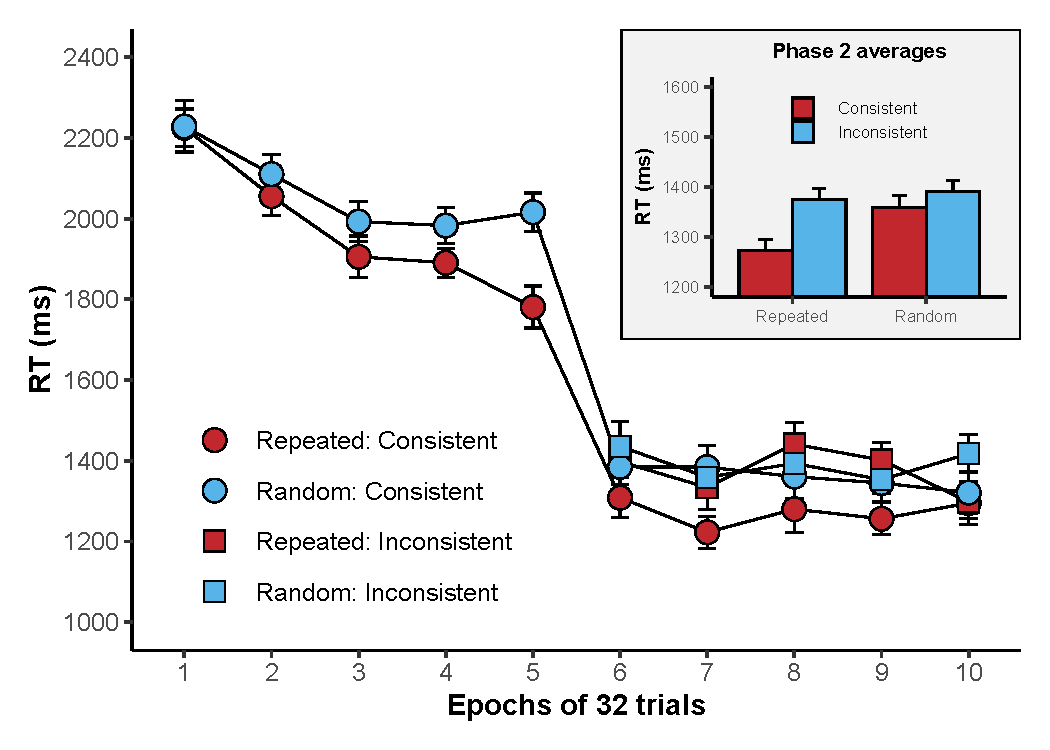
\includegraphics{CCC_ms1_files/figure-latex/Exp1-RT-figure-1} 

}

\caption{RT data for Experiment 1}\label{fig:Exp1-RT-figure}
\end{figure}

These data were explored with a Bayesian ANOVA, using the \emph{BayesFactor::anovaBF()} function (for all analyses in this study the priors were set at the default ``medium'' width). First taking the data from phase 1 (epochs 1-5), the model with the largest Bayes Factor (BF) contained the factors of epoch and configuration (repeated vs.~random), BF\textsubscript{10} = 2.4x10\textsuperscript{12} ± 9.8\%. The addition of the interaction term did not substantially improve the model fit, BF = 0.4 ± 9.92\%. The best fitting model was a better fit than the two models containing only one of the factors, smallest BF = 39.51 ± 9.83\%, providing significant support for the effects of configuration and epoch.

A Bayesian ANOVA on the data from phase 2 (epochs 6-10) found significant support for the model containing the factor of configuration, BF\textsubscript{10} = 89.41 ± 0.67\%. The next best fitting model contained the factor of epoch but was a substantially worse fit to the data, BF\textsubscript{10} = 0.02 ± 1.3\%. Thus there was considerable evidence for an effect of configuration, and evidence that there was no effect of epoch or an interaction between epoch and configuration.

To explore the differences in response times across the four trial types in phase 2, the data were averaged across the 5 epochs, and Bayesian t-tests were run using BayesFactor::ttestBF with the default Cauchy prior. This revealed support for a difference between the response times on ``repeated: consistent'' trials and those on the respective random trials (random: consistent), BF\textsubscript{10} = 4.14 ± 0\%. There was also evidence to suggest there was no difference between the response times for the ``repeated: inconsistent'' trials and the respective random trials, BF\textsubscript{10} = 0.24 ± 0.03\%. There was substantial support for a difference between the response times on repeated consistent and the repeated inconsistent trials, BF\textsubscript{10} = 7.87 ± 0\%.

\hypertarget{discussion}{%
\subsection{Discussion}\label{discussion}}

Experiment 1 sought to examine the consequence of an endogenous cue that prompts top-down control of the search process on contextual cuing. In phase 1 we established a robust contextual cuing effect. Following this, participants received instruction that each trial would be preceded by an arrow stimulus that would signal the side of the screen on which the target would appear. This cue was valid on all trials in phase 2. Consistent with these instructions and the processing of this cue, we observed substantially reduced search times in phase 2 compared to phase 1. The same set of repeated configurations were presented in Phase 2, but for half of the trials, the target was relocated to the diagonally opposed quadrant of the screen. Therefore, on these ``repeated inconsistent'' trials, the underlying configuration of distractors predicted the target in a location that opposed that of the (valid) endogenous cue. Across this phase we observed significant contextual cuing for the repeated consistent trials, demonstrating that the underlying configuration of distractors continued to guide attention in the presence of the endogenous cue. However, the repeated inconsistent trials did not lead to an impairment in response times relative to random trials, suggesting that the underlying configuration did not influence search on these trials.

\hypertarget{experiment-2}{%
\section{Experiment 2}\label{experiment-2}}

In Experiment 1 we demonstrated that an established effect of contextual cuing is maintained even when attention is being guided by the presence of a valid endogenous cue. That is, we found that the \emph{performance} of an established search behaviour in contextual cuing is not disrupted by concurrent top-down goals to guide attention in a controlled manner. In Experiment 2 we wanted to explore the \emph{learning} of the contextual cue itself, examining whether the presence of a valid endogenous cue may limit the development of a contextual cuing effect. To do this, we trained each participant on two sets of repeating configurations. One of these sets was always presented in the presence of a valid endogenous cue, while the other set was always presented in the absence of the endogenous cue. The extent to which there is a ``cue-competition'' effect between the endogenous cue and the contextual cues can be examined by comparing the contextual cuing effect we observe for the two sets of configurations. Given the clear difference in RTs we observed in Experiment 1 between the trials with the endogenous cue present and the cue being absent, we anticipated the same difference in responding in Experiment 2. Therefore we also included a second phase of Experiment 2 in which we removed the endogenous cue entirely from the task. This second phase therefore allowed us to directly compare the contextual cuing for the two sets of configurations when RTs were at a comparable level.

``Cue-competition'' effects have been examined previously in contextual cuing. Endo and Takeda (2004) trained participants with a contextual cuing task composed of distractor location configurations and repeating distractor identities. Their experiments suggested that the stronger configural (spatial) cue out-competed the cue provided by the distractor identities. Similarly, Kunar et al. (2014) found that when colour cues and configural cues both predicted the target location, configural cues were dominant and tended to overshadow the weaker colour cue. Beesley and Shanks (2012) looked at the cue-interaction effects \emph{within} a configuration of distractors. Participants were first trained with half a configuration of repeating distractors that predicted the target (8 out of 16 distractors). In a later stage these distractors were paired with a new half-configuration, such that the whole configuration now predicted the same target location. In contrast to the predictions of the vast majority of models of contingency learning, learning about these new predictive distractors was facilitated, rather than impaired in this second phase (relative to a control condition). Thus, Beesley and Shanks (2012) found that cue-competition was not observed within a configuration of equally predictive distractors. Together these studies suggest that the spatial configuration serves as a strong cue for the target and will out-compete non-configural cues for access to the learning mechanism. The dominance of the configuration in these situations may therefore lead to the prediction that the endogenous cue would not ``block'' the learning of the configuration in this task.

\hypertarget{method-1}{%
\subsection{Method}\label{method-1}}

\hypertarget{participants-1}{%
\subsubsection{Participants}\label{participants-1}}

Thirty-four undergraduate students from Lancaster University were recruited (mean age = 20.74, SD = 5.29; 28 identified as male and 6 as female) via the Psychology Research Participation System in the Department of Psychology at Lancaster University, in return for the opportunity to use the recruitment system for their own research in future years.

\hypertarget{materials-1}{%
\subsubsection{Materials}\label{materials-1}}

Participants were tested in a quiet laboratory testing cubicle, with a standard PC and a 24'' monitor set at a resolution of 1920 x 1080 pixels. All other materials and stimuli were identical to Experiment 1.

\hypertarget{design-1}{%
\subsubsection{Design}\label{design-1}}

Four repeated configurations were created in an identical manner to those used in Experiment 1. For each participant, two of these configurations were used for the ``cue-competition'' condition, in which the arrow cue was presented before the configuration, while two were used for the ``control'' condition (no arrow presented). As in Experiment 1, the four repeated configurations were paired with unique target positions from each of the four quadrants. We counterbalanced the use of the target quadrants across the factors of configuration type (repeated and random) and cue condition (cue-competition and control). For half of the participants, targets in the top left and bottom right were used for the repeated configurations presented with the arrow (cue-competition) condition, with targets in the top right and bottom left used for repeated configurations in the no-arrow (control) condition. For these participants, random configurations presented with the arrow had targets in the top right and bottom left, and random configurations without the arrow had targets in the top left and bottom right. For the other half of the participants these assignments were reversed (repeated-arrow: top-right and bottom-left; repeated-no arrow: top-left and bottom-right; random-arrow: top-left and bottom-right; random-no arrow: top-right and bottom-left).

\hypertarget{procedure-1}{%
\subsubsection{Procedure}\label{procedure-1}}

The procedure was the same as Experiment 1 with the following differences. Participants received 320 trials in total. For the first 160 trials, the arrow was presented for the relevant conditions. For the final 160 trials, the arrow was never presented. Rest breaks were given every 60 trials.

\hypertarget{results-1}{%
\subsection{Results}\label{results-1}}

Our criteria for removing outlier data were identical to Experiment 1. On average, trials ended with a timeout on 2.13\% of trials (SD = 1.83). Zero participants had an usually high proportion of timeouts. The mean accuracy of participants (not including timeout trials) was 95.85\% (SD = 6.10\%). One participant had an unusually low proportion of accurate trials and were removed from the sample. Zero participants were deemed to be an outlier in terms of mean RT.

For the remaining thirty-three participants we removed trials with a timeout and inaccurate trials, before removing outliers from the RT data. On average, the proportion of outliers removed was 2.81\% (SD = 1.04\%). One participant had an unusual proportion of trials removed as outlier RTs and were not included in the final analysis.

\begin{figure}

{\centering 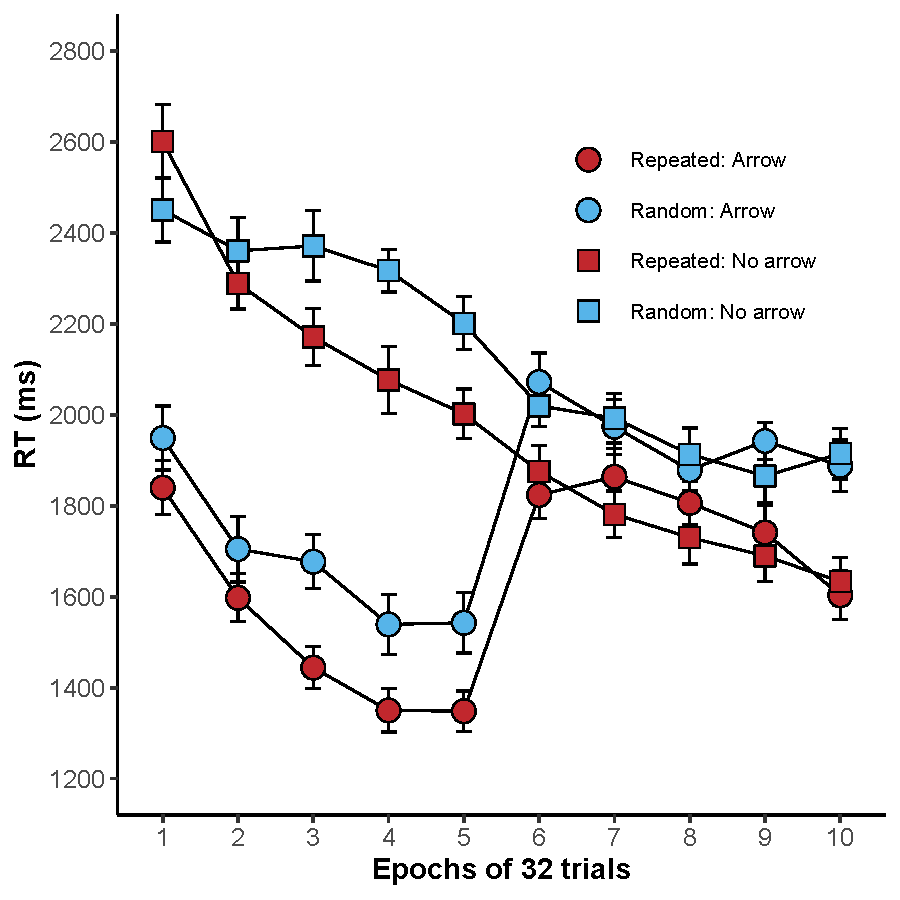
\includegraphics{CCC_ms1_files/figure-latex/Exp2-RT-figure-1} 

}

\caption{RT data for Experiment 2. Error bars show standard error of the mean on normalised data.}\label{fig:Exp2-RT-figure}
\end{figure}



Figure \ref{fig:Exp2-RT-figure} shows the RT data across the 10 epochs of the experiment. Contextual cuing emerged rapidly in both the arrow and no-arrow conditions, with little suggestion that the CC effect was different in the two conditions. The Phase 1 data were explored with a Bayesian ANOVA, which revealed that the best fitting model contained the factors of epoch, configuration (repeated vs.~random), and endogenous cue (arrow present vs.~arrow absent), with no interaction terms, BF\textsubscript{10} = 6.9x10\textsuperscript{100} ± 1.62\%. The next best fitting model contained all three factors and the interaction of epoch and configuration, BF\textsubscript{10} = 5.2x10\textsuperscript{100} ± 3.4\%, and this model was not a substantially worse fit to the data, BF = 0.75 ± 3.77\%. All other models were substantially worse fits than the best fitting model, largest BF = 0.25 ± 3.88\%. Importantly, the interaction term between the factors of endogenous cue and configuration did not improve the fit of the model, with support for the absence of this interaction, BF = 0.19 ± 2.48\%.

When the endogenous cue was removed in the second half of the experiment, RTs were equivalent across the two conditions. An effect of configuration was seen for both cuing conditions, with little discernible difference between the size of the cuing effects. We conducted a Bayesian ANOVA with factors of epoch, configuration and endogenous cue condition (arrow vs.~no-arrow). The best fitting model was that with just the factors of epoch and configuration with no interaction between the factors, BF\textsubscript{10} = 9.2x10\textsuperscript{14} ± 0.97\%. There was substantial support for this model over the next best fitting model, BF = 6.27 ± 28.25\%. To examine the interaction of the configuration and endogenous cue factors, we compared the model containing those two factors to the model containing the two factors plus the interaction of configuration and endogenous cue, which revealed support for the absence of an interaction, BF = 0.11 ± 3.42\%.

To provide further support for the absence of the interaction between the factors of configuration type and endogenous cue, the data from across the experiment (epochs 1-10) were analysed with a Bayesian ANOVA with only the factors of configuration and endogenous cue. The best fitting model was that with the two factors and no interaction, BF\textsubscript{10} = 3.6x10\textsuperscript{51} ± 1.67\%. The addition of the interaction term did not strengthen the model, with considerable support evident for the absence of the interaction, BF = 0.1 ± 3.56\%.

\hypertarget{discussion-1}{%
\subsection{Discussion}\label{discussion-1}}

Experiment 2 sought to examine whether the presence of a valid endogenous cue would impair the acquisition of a contextual cuing effect. In the first phase, two sets of configurations were trained, one of which was always presented in the presence of the endogenous cue, and one set which was presented without the endogenous cue. Overall there was considerable evidence that the cue was processed and acted upon, as response times to the target were much faster on cued trials. However, there was no evidence to suggest that this initial guidance of attention impaired the acquisition of the configurations on those trials. Furthermore, when the endogenous cue was never presented in the final phase of the experiment, the size of the contextual cuing effect was equivalent between the two sets of configurations; the Bayesian analyses found support for the equivalence of these CC effects.

The lack of competition effects seen in Experiment 2 are at odds with some findings in the CC literature (i.e., Endo \& Takeda, 2004; Kunar et al., 2014), where competition has been seen by more dominant or salient features of the displays. Instead, the findings point towards a more automatic nature to contextual cuing, whereby associations form ubiquitously, so long as they receive the focus of attention at some point within the search process (e.g., Beesley \& Shanks, 2012).

Taken together with the findings of Experiment 1, these data suggest that attention can be initially cued in an endogenous manner, before the underlying search configuration refines this attentional process to facilitate search for the target in repeated configurations. The equivalence of the CC effects in the two conditions (cued and uncued) suggests that the guidance by the context was driven largely (or perhaps entirely) by the distractors that appear close to the target. That is, while search times are longer in the uncued condition, and therefore more distractors are inevitably processed in this condition, this additional distractor processing does not result in stronger associative learning. Experiment 3 explored this hypothesis.

\hypertarget{experiment-3}{%
\section{Experiment 3}\label{experiment-3}}

Existing data from studies of contextual cuing has pointed towards a localised learning effect for repeated configurations, with those distractors closest to the target being preferentially weighted in the learning process over those located further from the target. For example, Olson and Chun (2002) trained participants with three sets of repeating configurations that differed in terms of which distractors repeated across trials. For one set, the entire global context (all of the distractors) repeated, while for the other two sets only the short-range (those close to the target) or the long-range distractors (those far from the target) repeated across trials. They found no difference between the CC effect in the short-range and global configurations, while the CC effect was not significant for the long-range context. Similar results have been shown by Brady and Chun (2007) which led to the development of the spatial constraints model of contextual cuing, in which distractor-target associations occurring in close proximal space are weighted more heavily in the learning process (over those occurring across greater spatial distance).

It is important to consider how the bias towards local learning may interact with the attentional scanning process during contextual cuing. The analysis of eye-movements during contextual cuing tasks (Beesley et al., 2018; Tseng \& Li, 2004) has revealed a characteristic scanning pattern comprising two phases: search initially occurs in a seemingly random manner, as the eyes move between distractors in the central region of the distractor field, before then moving in a more directed manner towards the target position. Contextual cuing appears to result from a cessation of the first (random) search phase at an earlier time point in the entire search process, such that processing of repeated distractors will, on average, result in fewer fixations. With respect to the current study, in Experiments 1 and 2 we have initially directed attention towards the side of the screen that contains the target on cued trials. This will bring about an early cessation of the first phase of the search process. From here, however, it seems that eye-movements are still facilitated by the repetition of the context.

To test this characterisation of the interaction between the endogenous cue and the repeated context, we exposed participants to the same procedure as used in phase 1 of Experiment 1, which establishes a contextual cuing effect prior to the use of the endogenous cue. In a second phase we then presented the endogenous cue on every trial (as in Experiment 1), but we manipulated the presence of the repeated distractors within the configurations. For each repeated configuration we created two variations: in the ``proximal'' configurations, only the distractors in the quadrant containing the target match those from the full repeated configuration, while the distractors in the other three quadrants were randomly arranged on each trial; in the ``distal'' configurations, the distractors closest to the target were randomised, while the distractors in the other three quadrants were the same as those in the full repeated configuration. During this phase we also presented fully repeated configurations and fully randomised configurations. Comparison of the response times across these four trial types will allow us to determine the contribution of proximal and distal distractors to the CC effect in this task.

\hypertarget{method-2}{%
\subsection{Method}\label{method-2}}

\hypertarget{participants-2}{%
\subsubsection{Participants}\label{participants-2}}

Forty-two undergraduate students from Lancaster University were recruited (mean age = 18.64, SD = 2.84; 28 identified as male and 12 as female) via the Psychology Research Participation System in the Department of Psychology at Lancaster University, in return for the opportunity to use the recruitment system for their own research in future years.

\hypertarget{materials-2}{%
\subsubsection{Materials}\label{materials-2}}

The experiment was conducted in a quiet testing cubicle, as described in Experiment 2. All other materials and stimuli were identical to Experiment 1.

\hypertarget{design-2}{%
\subsubsection{Design}\label{design-2}}

The design of phase 1 was identical to Experiment 1, with four repeated configurations created and presented with random configurations during this phase. For Phase 2, each of the four configurations was manipulated to create two alternative conditions. In the ``Repeated distal'' condition, the four distractors in the target quadrant were randomly arranged on each trial, while the 12 distractors in the other three quadrants were presented in the same positions as had been trained in Phase 1. Thus, slower response times for this condition (compared to the fully repeated configurations) would indicate the extent to which participants CC was governed by the distractors closest to the target. For the ``Repeated proximal'' condition, the four distractors in the target quadrant were presented in the same positions as had been trained in Phase 1, while the 12 distractors in the other three quadrants were randomly arranged on each trial. Thus, slower response times for this condition (compared to the fully repeated configurations) would indicate the extent to which CC was governed by the distractors further from the target. Comparison of the RTs for these different configurations with those of the random configurations would allow for the assessment of whether these subsets of distractors had \emph{any} contribution to the CC effect that had developed during phase 1.

\hypertarget{procedure-2}{%
\subsubsection{Procedure}\label{procedure-2}}

The procedure was identical to Experiment 1.

\hypertarget{results-2}{%
\subsection{Results}\label{results-2}}

Our criteria for removing outlier data were identical to Experiment 1. On average, trials ended with a timeout on 2.81\% (SD = 2.25) of trials . Two participants had an usually high proportion of timeouts and were removed from the sample. The mean accuracy of participants (not including timeout trials) was 96.09\% (SD = 8.57\%). Two participants that had an unusually low proportion of accurate trials and were also removed. Zero participants were deemed to be an outlier in terms of mean RT.

For the remaining thirty-eight participants we removed trials with a timeout and inaccurate trials, before removing outliers from the RT data. On average, the proportion of outliers removed was 3.17\% (SD = 0.71\%). Zero participants had an unusual proportion of trials removed as outlier RTs.

\begin{figure}

{\centering 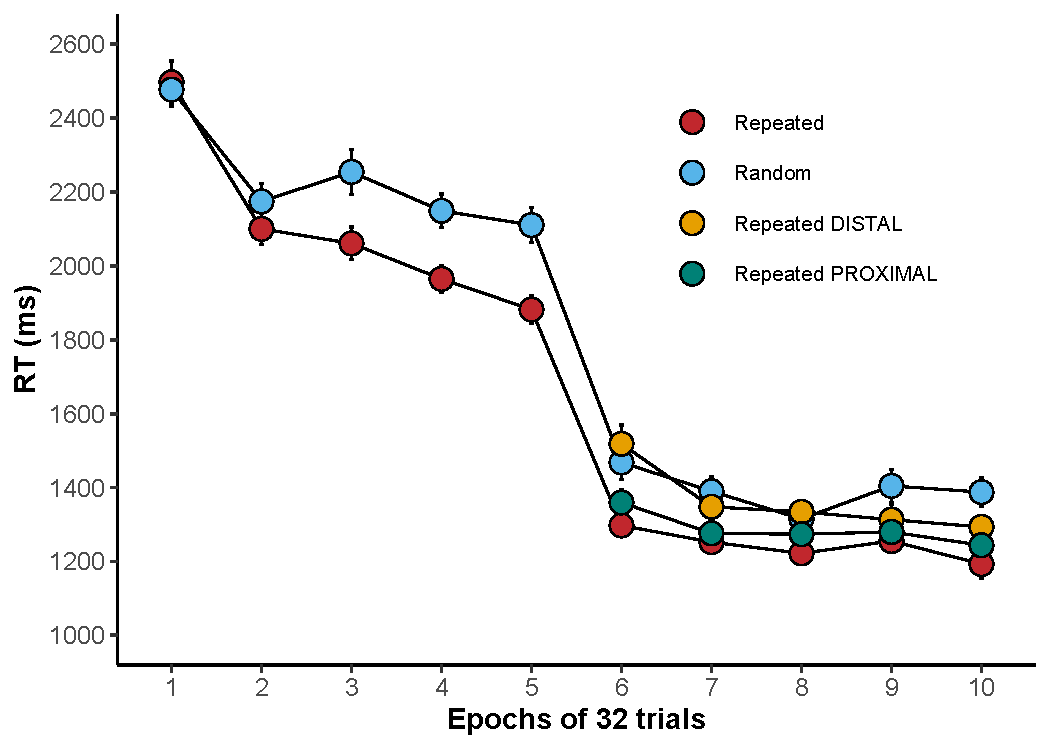
\includegraphics{CCC_ms1_files/figure-latex/Exp3-RT-figure-1} 

}

\caption{(ref:Exp3-RT-figure)}\label{fig:Exp3-RT-figure}
\end{figure}

Figure \ref{fig:Exp3-RT-figure} shows the RT data across the 10 epochs of Experiment 3. As in Experiment 1, contextual cuing was readily established in Phase 1. These data were subjected to a Bayesian ANOVA which revealed that the best fitting model contained the factors of configuration (repeated vs.~random) and epoch, and an interaction between those factors, BF\textsubscript{10} = 5.5x10\textsuperscript{24} ± 2.71\%. However, the model without the interaction provided a strong fit to the data, BF\textsubscript{10} = 5x10\textsuperscript{24} ± 1\%, and a comparison between the two models did not find significant evidence in support of the interaction term, BF = 0.92 ± 2.89\%. The best fitting model was substantially supported over the remaining models, smallest BF = 3993.8 ± 2.8\%, providing considerable support for the factors of epoch and configuration.

The response times decreased significantly with the presentation of the valid endogenous cue in Phase 2. Response times to the fully repeated configurations were somewhat comparable to those when just the proximal repeated distractors were present. Response times for the distal repeated distractors appeared to be slower and comparable to the fully random configurations. The Phase 2 data were subjected to a Bayesian ANOVA which found that the best fitting model contained the factors of configuration and epoch but no interaction between the factors, BF\textsubscript{10} = 1.4x10\textsuperscript{14} ± 0.93\%. This model provided a superior fit to the data compared to the next best fitting model that included the two factors and the interaction term, BF = 119.72 ± 2.36\%, providing strong support for the contribution of the two factors and the absence of an interaction between the two factors.

\begin{figure}

{\centering 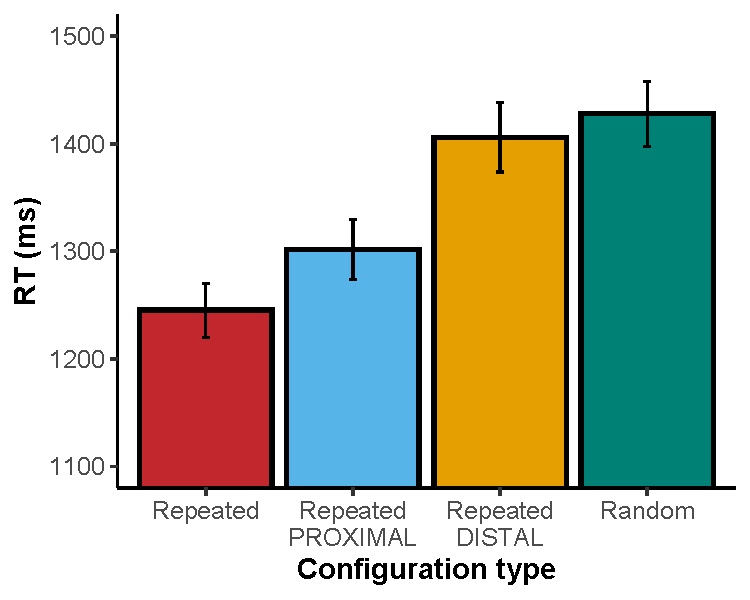
\includegraphics{CCC_ms1_files/figure-latex/Exp3-Phase-2-figure-1} 

}

\caption{RT data for phase 2 of Experiment 3. Error bars show standard error of the mean on normalised data.}\label{fig:Exp3-Phase-2-figure}
\end{figure}



Figure \ref{fig:Exp3-Phase-2-figure} shows the mean RTs to the four types of configuration, averaged across the 5 epochs of Phase 2 (see the Appendix for a plot of these data showing the distribution of individual data points for RT differences). To explore the differences in response times Bayesian t-tests were run for all pairwise comparisons using BayesFactor::ttestBF with the default Cauchy prior. The response times to repeated and repeated-proximal configurations were both faster than those to random configurations, smallest BF\textsubscript{10} = 10313.81 ± 0\%. In contrast, there was no evidence that the response times to repeated-distal configurations were different from those to random configurations, BF\textsubscript{10} = 0.39 ± 0.04\%. Response times to repeated configurations were faster than those to repeated-proximal configurations, BF\textsubscript{10} = 4.67 ± 0\%. Response times to repeated-proximal configurations were faster than those to repeated-distal configurations, BF\textsubscript{10} = 31.88 ± 0\%.

\hypertarget{discussion-2}{%
\subsection{Discussion}\label{discussion-2}}

Experiment 3 explored the localisation of the distractors driving contextual cuing when attention is guided initially by an endogenous cue. As expected, there was substantial evidence that contextual cuing was present when the distractors close to the target were maintained, but not when these distractors were randomly arranged. These data provide confirmatory evidence for the hypothesised interplay between the two drivers of attention: initially attention is guided by the endogenous cue towards one half of the screen. Despite visual search never commencing in this manner in the first half of the experiment, a CC effect was readily observed, but only for those configurations in which the local distractors were present. Thus it seems that the stored representations of configurations surrounding target positions are very flexibly deployed in visual search. These data lend support to the notion that the effect of the repeated configuration comes late on in the visual search process, and that each trial commences with a random search process that is not guided by the repeated configuration (Beesley et al., 2018; Tseng \& Li, 2004).

\hypertarget{general-discussion}{%
\section{General Discussion}\label{general-discussion}}

Three experiments explored the impact of a central endogenous cue on the contextual cuing of visual search. In Experiment 1, having established a contextual cuing effect, each trial was preceded by an central endogenous cue of attention in the form of an arrow, directing attention towards the side of the screen in which the target was positioned (this arrow cue was always valid in each of the three experiments). Despite participants clearly using this cue, visual search was still facilitated by the presence of the repeating pattern of visual search. This experiment demonstrated that, once acquired, the activation of the memory representation and its impact on performance of visual search remains intact in the presence of a top-down instruction to guide attention. Experiment 2 examined the storage of these contextual representations, and whether these were impaired by an endogenous cue guiding search. We found equivalent levels of contextual cuing for two sets of configurations, one of which was paired with the cue and one which was not. Together, these two experiments suggest a seamless interplay between these two factors governing attention in visual search: the endogenous cue initially guides attention and the repeated configuration continues to refine and guide attention towards a fixation on the target. In Experiment 3 we therefore explored whether the localised distractors around the target were sufficient to generate CC following the guidance by the endogenous cue. Indeed, the CC effect was as large in the case of the proximal distractors compared to the entire repeated configuration of distractors. In contrast, those repetitions that did not contain the proximal distractors failed to generate a CC effect.

The effect of CC on visual search has frequently been characterised as an automatic influence on behaviour (e.g., Chun \& Jiang, 1998; Chun \& Nakayama, 2000; Geyer et al., 2021). This characterisation of CC comes from multiple aspects of the observed effect. Updating of the associations is somewhat slow and seemingly inflexible to changes in the acquired associations (Makovski \& Jiang, 2011; Manginelli \& Pollmann, 2009; Zellin et al., 2013; e.g., \textbf{zellin2011?}), and therefore perhaps reflects a habitual form of behaviour. In addition, contextual cuing has frequently been observed in the absence of above-chance recognition memory for the repeating search configurations (e.g., Colagiuri \& Livesey, 2016), which suggests a non-conscious, automatically evoked form of behaviour. Despite this persistent characterisation, the automaticity (or controllability) of CC has rarely been directly tested in the literature. To our knowledge, only the experiments of Luque and colleagues (Luque et al., 2017; Luque et al., 2021) have directly assessed this aspect of CC, by placing the influence of the configuration in competition with top-down goals in the task. Their findings supported the conclusion that CC performance can be controlled and will not guide search for the target when another aspect of the task governs attentional control. In the current study, the repeated configurations continued to have an influence on search performance even when attention had been guided by the endogenous cue. These results are therefore somewhat at odds with the conclusions of Luque and colleagues (Luque et al., 2017; Luque et al., 2021).

To what extent is this behaviour best characterised as ``automatic'' in nature? Arguably the clearest demonstration of an automatic effect of a stimulus on behaviour is when the associated behaviour is elicited even when it is counter-productive to the current goals {[}ref{]}. Such a test was constructed in the repeated inconsistent trials of Experiment 1, in which the repeated configuration was associated with a target appearing in a position that was in the opposite side of the screen to the direction of the endogenous cue. If the repeated configuration was having an effect on behaviour on these trials we would have expected to see slower response times compared to random trials. This was not the case: response times were equivalent in the two conditions. As such it has hard to claim here that the configuration is having an \emph{automatic} effect on behaviour, according to this strict characterisation of such an effect. Nevertheless, the experiments here reveal an interplay between top-down processes and stimulus driven effects on attention in CC.

The current data reveal that the influence of repeated contexts has a relatively late control on behaviour in visual search. Previous analysis of eye-movements during CC (Beesley et al., 2018; Tseng \& Li, 2004) has shown that contextual cuing (and visual search more generally) has two characteristic components. The first of these is an inefficient search process where search fails to move towards the target in
trials with more fixations. This is followed by a phase in which monotonic, positive increments are made toward the target position in the final 3 to 4 fixations. CC reduces the frequency of trials with the initial (random) search period (there are more of such trials for random configurations and fewer for repeated configurations). Thus, the effect of the endogenous central cue in the current study is to eliminate, or considerably reduce, the engagement with this first phase of the search process. The results of this study strongly imply that the positive associative information in the repeating configurations is extracted in the final stages of search and is localised to the target. This true both in terms of the performance of an acquired configuration (Experiments 1 and 3) and the acquisition of the representation for that configuration (Experiment 2). Perhaps paradoxically, the benefit of repeated configurations in search occurs shortly before the target is fixated.

In conclusion\ldots.

\newpage

\hypertarget{appendix}{%
\section{Appendix}\label{appendix}}

\begin{figure}

{\centering 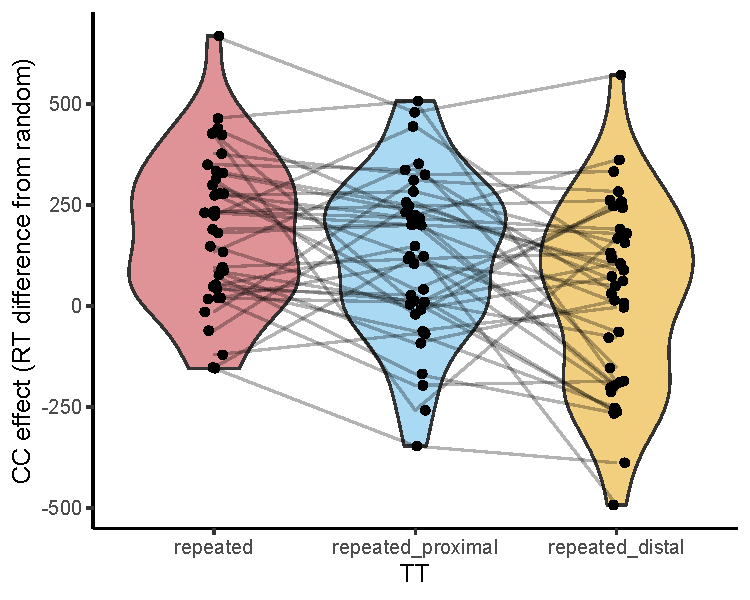
\includegraphics{CCC_ms1_files/figure-latex/Exp3-Phase-2-RTdiff-figure-1} 

}

\caption{(ref:Exp3-Phase-2-RTdiff-figure)}\label{fig:Exp3-Phase-2-RTdiff-figure}
\end{figure}

RT data for phase 2 of Experiment 3. Error bars show standard error of the mean on normalised data. The distribution of RT data for phase 2 of Experiment 3, plotted as difference scores (RT to random configurations minus RT to repeated configuration type). Individual points are presented and linked across trial types.

\newpage

\hypertarget{references}{%
\section*{References}\label{references}}
\addcontentsline{toc}{section}{References}

\hypertarget{refs}{}
\begin{CSLReferences}{1}{0}
\leavevmode\vadjust pre{\hypertarget{ref-beesley2018}{}}%
Beesley, T., Hanafi, G., Vadillo, M. A., Shanks, David. R., \& Livesey, E. J. (2018). Overt attention in contextual cuing of visual search is driven by the attentional set, but not by the predictiveness of distractors. \emph{Journal of Experimental Psychology: Learning, Memory, and Cognition}, \emph{44}(5), 707--721. \url{https://doi.org/10.1037/xlm0000467}

\leavevmode\vadjust pre{\hypertarget{ref-beesley2012}{}}%
Beesley, T., \& Shanks, D. R. (2012). Investigating cue competition in contextual cuing of visual search. \emph{Journal of Experimental Psychology: Learning, Memory, and Cognition}, \emph{38}(3), 709--725. \url{https://doi.org/10.1037/a0024885}

\leavevmode\vadjust pre{\hypertarget{ref-beesley2015b}{}}%
Beesley, T., Vadillo, M. A., Pearson, D., \& Shanks, D. R. (2015). Pre-exposure of repeated search configurations facilitates subsequent contextual cuing of visual search. \emph{Journal of Experimental Psychology: Learning, Memory, and Cognition}, \emph{41}(2), 348--362. \url{https://doi.org/10.1037/xlm0000033}

\leavevmode\vadjust pre{\hypertarget{ref-beesley2016}{}}%
Beesley, T., Vadillo, M. A., Pearson, D., \& Shanks, D. R. (2016). Configural learning in contextual cuing of visual search. \emph{Journal of Experimental Psychology: Human Perception and Performance}, \emph{42}(8), 1173--1185. \url{https://doi.org/10.1037/xhp0000185}

\leavevmode\vadjust pre{\hypertarget{ref-brady2007}{}}%
Brady, T. F., \& Chun, M. M. (2007). Spatial constraints on learning in visual search: {Modeling} contextual cuing. \emph{Journal of Experimental Psychology: Human Perception and Performance}, \emph{33}(4), 798--815. \url{https://doi.org/10.1037/0096-1523.33.4.798}

\leavevmode\vadjust pre{\hypertarget{ref-chun1998}{}}%
Chun, M. M., \& Jiang, Y. (1998). Contextual {Cueing}: {Implicit Learning} and {Memory} of {Visual Context Guides Spatial Attention}. \emph{Cognitive Psychology}, \emph{36}(1), 28--71. \url{https://doi.org/10.1006/cogp.1998.0681}

\leavevmode\vadjust pre{\hypertarget{ref-chun2000a}{}}%
Chun, M. M., \& Nakayama, K. (2000). On the {Functional Role} of {Implicit Visual Memory} for the {Adaptive Deployment} of {Attention Across Scenes}. \emph{Visual Cognition}, \emph{7}(1-3), 65--81. \url{https://doi.org/10.1080/135062800394685}

\leavevmode\vadjust pre{\hypertarget{ref-colagiuri2016}{}}%
Colagiuri, B., \& Livesey, E. J. (2016). Contextual cuing as a form of nonconscious learning: {Theoretical} and empirical analysis in large and very large samples. \emph{Psychonomic Bulletin \& Review}, \emph{23}(6), 1996--2009. \url{https://doi.org/10.3758/s13423-016-1063-0}

\leavevmode\vadjust pre{\hypertarget{ref-cousineau2005}{}}%
Cousineau, D. (2005). Confidence intervals in within-subject designs: {A} simpler solution to {Loftus} and {Masson}'s method. \emph{Tutorials in Quantitative Methods for Psychology}, \emph{1}(1), 42--45. \url{https://doi.org/10.20982/tqmp.01.1.p042}

\leavevmode\vadjust pre{\hypertarget{ref-endo2004}{}}%
Endo, N., \& Takeda, Y. (2004). Selective learning of spatial configuration and object identity in visual search. \emph{Perception \& Psychophysics}, \emph{66}(2), 293--302. \url{https://doi.org/10.3758/BF03194880}

\leavevmode\vadjust pre{\hypertarget{ref-geyer2021}{}}%
Geyer, T., Seitz, W., Zinchenko, A., Müller, H. J., \& Conci, M. (2021). Why {Are Acquired Search-Guiding Context Memories Resistant} to {Updating}? \emph{Frontiers in Psychology}, \emph{12}, 650245. \url{https://doi.org/10.3389/fpsyg.2021.650245}

\leavevmode\vadjust pre{\hypertarget{ref-kunar2007}{}}%
Kunar, M. A., Flusberg, S., Horowitz, T. S., \& Wolfe, J. M. (2007). Does contextual cuing guide the deployment of attention? \emph{Journal of Experimental Psychology: Human Perception and Performance}, \emph{33}(4), 816--828. \url{https://doi.org/10.1037/0096-1523.33.4.816}

\leavevmode\vadjust pre{\hypertarget{ref-kunar2014}{}}%
Kunar, M. A., John, R., \& Sweetman, H. (2014). A configural dominant account of contextual cueing: {Configural} cues are stronger than colour cues. \emph{Quarterly Journal of Experimental Psychology (2006)}, \emph{67}(7), 1366--1382. \url{https://doi.org/10.1080/17470218.2013.863373}

\leavevmode\vadjust pre{\hypertarget{ref-luque2021}{}}%
Luque, D., Beesley, T., Molinero, S., \& Vadillo, M. A. (2021). Contextual cuing of visual search does not guide attention automatically in the presence of top-down goals. \emph{Journal of Experimental Psychology: Human Perception and Performance}, \emph{47}(8), 1080--1090. \url{https://doi.org/10.1037/xhp0000930}

\leavevmode\vadjust pre{\hypertarget{ref-luque2017b}{}}%
Luque, D., Vadillo, M. A., Lopez, F. J., Alonso, R., \& Shanks, D. R. (2017). Testing the controllability of contextual cuing of visual search. \emph{Scientific Reports}, \emph{7}(1), 39645. \url{https://doi.org/10.1038/srep39645}

\leavevmode\vadjust pre{\hypertarget{ref-makovski2017}{}}%
Makovski, T. (2017). Learning {``{What}''} and {``{Where}''} in {Visual Search}. \emph{Japanese Psychological Research}, \emph{59}(2), 133--143. \url{https://doi.org/10.1111/jpr.12146}

\leavevmode\vadjust pre{\hypertarget{ref-makovski2018}{}}%
Makovski, T. (2018). Meaning in learning: {Contextual} cueing relies on objects' visual features and not on objects' meaning. \emph{Memory \& Cognition}, \emph{46}(1), 58--67. \url{https://doi.org/10.3758/s13421-017-0745-9}

\leavevmode\vadjust pre{\hypertarget{ref-makovski2011}{}}%
Makovski, T., \& Jiang, Y. V. (2011). Investigating the {Role} of {Response} in {Spatial Context Learning}. \emph{Quarterly Journal of Experimental Psychology}, \emph{64}(8), 1563--1579. \url{https://doi.org/10.1080/17470218.2011.564291}

\leavevmode\vadjust pre{\hypertarget{ref-manginelli2009}{}}%
Manginelli, A. A., \& Pollmann, S. (2009). Misleading contextual cues: {How} do they affect visual search? \emph{Psychological Research}, \emph{73}(2), 212--221. \url{https://doi.org/10.1007/s00426-008-0211-1}

\leavevmode\vadjust pre{\hypertarget{ref-olson2002}{}}%
Olson, I. R., \& Chun, M. M. (2002). Perceptual constraints on implicit learning of spatial context. \emph{Visual Cognition}, \emph{9}(3), 273--302. \url{https://doi.org/10.1080/13506280042000162}

\leavevmode\vadjust pre{\hypertarget{ref-sewell2018}{}}%
Sewell, D. K., Colagiuri, B., \& Livesey, E. J. (2018). Response time modeling reveals multiple contextual cuing mechanisms. \emph{Psychonomic Bulletin \& Review}, \emph{25}(5), 1644--1665. \url{https://doi.org/10.3758/s13423-017-1364-y}

\leavevmode\vadjust pre{\hypertarget{ref-smyth2008}{}}%
Smyth, A. C., \& Shanks, D. R. (2008). Awareness in contextual cuing with extended and concurrent explicit tests. \emph{Memory \& Cognition}, \emph{36}(2), 403--415. \url{https://doi.org/10.3758/MC.36.2.403}

\leavevmode\vadjust pre{\hypertarget{ref-tseng2004}{}}%
Tseng, Y.-C., \& Li, C.-S. R. (2004). Oculomotor correlates of context-guided learning in visual search. \emph{Perception \& Psychophysics}, \emph{66}(8), 1363--1378. \url{https://doi.org/10.3758/BF03195004}

\leavevmode\vadjust pre{\hypertarget{ref-vadillo2016}{}}%
Vadillo, M. A., Konstantinidis, E., \& Shanks, D. R. (2016). Underpowered samples, false negatives, and unconscious learning. \emph{Psychonomic Bulletin \& Review}, \emph{23}(1), 87--102. \url{https://doi.org/10.3758/s13423-015-0892-6}

\leavevmode\vadjust pre{\hypertarget{ref-vickery2005}{}}%
Vickery, T. J., King, L.-W., \& Jiang, Y. (2005). Setting up the target template in visual search. \emph{Journal of Vision}, \emph{5}(1), 8. \url{https://doi.org/10.1167/5.1.8}

\leavevmode\vadjust pre{\hypertarget{ref-vo2012}{}}%
Võ, M. L.-H., \& Wolfe, J. M. (2012). When does repeated search in scenes involve memory? {Looking} at versus looking for objects in scenes. \emph{Journal of Experimental Psychology. Human Perception and Performance}, \emph{38}(1), 23--41. \url{https://doi.org/10.1037/a0024147}

\leavevmode\vadjust pre{\hypertarget{ref-zellin2013}{}}%
Zellin, M., von Muhlenen, A., Muller, H. J., \& Conci, M. (2013). Statistical learning in the past modulates contextual cueing in the future. \emph{Journal of Vision}, \emph{13}(3), 19--19. \url{https://doi.org/10.1167/13.3.19}

\end{CSLReferences}


\end{document}
